\section{Experimental Evaluation}
\label{sec:experiments}

%%SL.5.24: For the sake of space, I think we can cut this and the subsection headings, and things are still mostly readable.
%The goal of our empirical evaluation is to study and compare the performance of CQL to prior offline RL methods on a wide range of domains and dataset compositions. We evaluate CQL along  multiple axes: the complexity of the underlying control problem, the way that the offline data is collected, and with both low-dimensional state and high-dimensional image inputs. 

% Additionally, we also evaluate CQL as an off-policy evaluation (OPE) method on the high-dimensional MuJoCo benchmark tasks, which typically pose a major challenge for modern OPE methods~\citep{nachum2019dualdice}. 

% Finally, we aim to analyze different components of CQL, highlighting the significance and empirical effects of the different design choices discussed in Section~\ref{sec:framework}.

%\subsection{Offline RL in Continuous Control Domains}
We compare CQL to prior offline RL methods on a range of domains and dataset compositions, including continuous and discrete action spaces, state observations of varying dimensionality, and high-dimensional image inputs. We first evaluate actor-critic CQL, using CQL($\mathcal{H}$) from Algorithm~\ref{alg:practical_alg}, on continuous control datasets from the D4RL benchmark~\citep{d4rl}.
%%SL.5.24: Something to be careful of: make sure we don't violate anonymity by using a version of D4RL that is newer than what is actually released! You may want to coordinate with Justin to get the D4RL paper updated (though if it's updated just days before, that's also a bit awkward).
We compare to: prior offline RL methods that use a policy constraint -- BCQ~\citep{fujimoto2018off}, BEAR~\citep{kumar2019stabilizing} and BRAC~\citep{wu2019behavior}; standard SAC~\citep{haarnoja}, an off-policy actor-critic method that we adapt to offline setting; and a behavioral cloning (BC) baseline that imitates the data distribution. 
% We also ran AlgeaDICE~\citep{nachum2019algaedice}, a method that uses a state-marginal constraint, using code released by the authors, but were unable to get it to improve over a random initialization on any of the tasks, as learning was unstable and diverged quickly, and we provide these learning curves in Appendix~\ref{app:additional_results}.
%%SL.5.24: For AlgeaDICE, I still think these sentences are damn awkward. If you really want to have this, maybe rephrase more briefly: We also attempted to run AlgeaDICE~\citep{} on these tasks, but were unable to obtain reasonable results with the authors' code (more details in Appendix~\ref{app:additional_results}). [I would also recommend omitting this sentence in the arxiv and only including it in the submission copy for the reviewers!]
% done, removed
%%SL.5.11: Could we add a comparison to AWR? I feel like this would not only make the results more complete, but also help to "legitimize" the viability of AWR as an offline RL algorithm. I think many readers of the original paper might have missed that AWR is also a good offline RL method, and by not comparing to it here, we in some sense reinforce that notion.
%%AK.5.13: TODO in the D4RL paper

\begin{table*}[h]
\centering
%\scriptsize
\fontsize{8}{8}\selectfont

\begin{tabular}{l|r|r|r|r|r|r||r}
\hline
\textbf{Task Name} & \textbf{SAC} & \textbf{BC} & \textbf{BCQ} & \textbf{BEAR} & \textbf{BRAC-p} & \textbf{BRAC-v} & \textbf{CQL($\mathcal{H}$)}\\ \hline
halfcheetah-random &  2.1 & 30.5 & 2.2 & 25.5 & 23.5 & 28.1 & \textbf{35.4} \\
hopper-random & 9.8 & \textbf{11.3} & 9.2 & 9.5 & \textbf{11.1} & \textbf{12.0} & \textbf{10.8}\\
walker2d-random & 1.6 & 4.1 & 4.8 &  \textbf{6.7} & 0.8 & 0.5 & \textbf{7.0}\\ \hline
halfcheetah-medium & -4.3 & 36.1 & 35.4 & 38.6 & \textbf{44.0} & \textbf{45.5} & \textbf{44.4}\\
walker2d-medium & 0.9 & 6.6 & 19.2 & 33.2 & 72.7 & \textbf{81.3} & {79.2}\\
hopper-medium & 0.8 & 29.0 & 37.1 & 47.6 & 31.2 & 32.3 & \textbf{65.2}\\ \hline
halfcheetah-expert & -1.9 & \textbf{107.0} & \textbf{106.0} & \textbf{108.2} & 3.8 & -1.1 & {104.8}\\
hopper-expert & 0.7 & \textbf{109.0} & \textbf{107.6} & \textbf{110.3} & 6.6 & 3.7 & \textbf{109.9} \\
walker2d-expert & -0.3 & 125.7 & 128.5 & 106.1 & -0.2 & -0.0 & \textbf{153.9} \\ \hline
halfcheetah-medium-expert & 1.8 & 35.8 & 59.2 & 51.7 & 43.8 & 45.3 & \textbf{62.4}\\
walker2d-medium-expert & 1.9 & 11.3 & 19.1 & 10.8 & -0.3 & 0.9 & \textbf{98.7}\\
hopper-medium-expert & 1.6 & \textbf{111.9} & 66.6 & 4.0 & 1.1 & 0.8 & \textbf{111.0}\\ \hline
halfcheetah-random-expert & 53.0 & 1.3 & 59.6 & 24.6 & 30.2 & 2.2 & \textbf{92.5}\\
walker2d-random-expert & 0.8 & 0.7 & 0.0 & 1.9 & 0.2 & 2.7 & \textbf{91.1}\\
hopper-random-expert & 5.6 & 10.1 & 9.8 & 10.1 & 5.8 & 11.1 & \textbf{110.5} \\ \hline
% hopper-random-expert & 160.2 & 309.5 & 298.5 & 307.6 & 167.3 & 342.1 & 3576.2 \\ \hline
%%SL.5.27: Make sure these are in normalized scores (I think this is raw reward?)
halfcheetah-mixed & -2.4 & 38.4 & 29.5 & 36.2 & \textbf{45.6} & \textbf{45.9} & \textbf{46.2}\\
hopper-mixed & 3.5 & 11.8 & 15.7 & 25.3 & 0.7 & 0.8 & \textbf{70.3}\\
walker2d-mixed & 1.9 & 11.3 & 8.3 & 10.8 & -0.3 & 0.9 & \textbf{33.4}\\
\hline
\end{tabular}
\caption{\label{table:mujoco}{\small Performance of CQL($\mathcal{H}$) and prior methods on MuJoCo tasks from D4RL, on the normalized return metric. Note that CQL performs similarly or better than the best prior method with simple datasets, and greatly outperforms prior methods with complex distributions (``--mixed'', ``--random-expert'', ``--medium-expert'').}}
\normalsize
\vspace{-10pt}
\end{table*}

% halfcheetah-random & -17.9 & 3502.0 & -2.1 & 2885.6 & 2641.0 & 3207.3 & \textbf{4524.7} \\
% halfcheetah-medium &  4196.4 & -808.6 & 4117.0 & 4508.7 & \textbf{5178.2} & \textbf{5365.3} & \textbf{5281.6} \\
% halfcheetah-mixed &  4492.1 & -581.3 & 3377.2 & 4211.3 & \textbf{5384.7} & \textbf{5413.8} & \textbf{5476.3}\\
% halfcheetah-medium-expert &  4169.4 & -55.7 &  7415.6 & 6132.5 & 5156.0 & 5342.4 & \textbf{9025.0}\\
% halfcheetah-random-expert &  -113.1 & 6298.7 & 7161.3 & 2768.8 & 3465.2 & -9.55 & \textbf{7951.9}\\ 
% \hline
% walker2d-random & 73.0 & 192.0 & 266.9 & 307.6 & 38.4 & 23.9 & \textbf{323.1}\\
% walker2d-medium & 304.8 & 44.2 & 881.7 & 1526.7 & 3341.1 & \textbf{3734.4} & \textbf{3801.4} \\
% walker2d-mixed & 518.6 & 87.8 & 384.6 & 495.3 & -11.5 & 44.5 & \textbf{1391.0} \\
% walker2d-medium-expert & 297.0 & -5.1 & 876.7 & 1193.6 & 141.7 & 3058.9 & \textbf{4348.1} \\
% walker2d-random-expert & 33.5 & 37.1 &  & 88.9 & 12.1 & 124.9 & \textbf{4245.8} \\
% \hline
% hopper-random & 299.4 & 347.7 & 274.7 & 289.5 & \textbf{341.0} & \textbf{370.5} & \textbf{355.2} \\
% hopper-medium & 923.5 & 5.7 & 1186.7 & 1527.9 & 994.8 & 1030.0 & \textbf{2403.1}\\
% hopper-mixed & 364.4 & 93.3 & 491.3 & 802.7 & 2.0 & 5.3 & \textbf{2267.9}\\
% hopper-medium-expert & \textbf{3621.2} & 32.9 & 2146.8 & 109.8 & 16.0 & 5.1 & \textbf{3699.1}\\
% \hline
% ant-random & & & & & & & 932.4\\
% ant-medium & & & & & & & 3325.4 \\
% ant-mixed & & & & & & & 2973.8\\
% ant-medium-expert & & & & & & & 3400.1 \\
% ant-random-expert & & & & & & & 2309.3\\
% \hline

Results for the simpler gym domains are shown in Table~\ref{table:mujoco}. The results for BEAR, BRAC and BC are based on numbers reported by \citet{d4rl}. On the datasets generated from a single policy, marked as ``-random'', ``-expert'' and ``-medium'', CQL matches or exceeds the best prior methods, but by a small margin. However, on datasets that combine multiple policies (``-mixed'', ``-medium-expert'' and ``-random-expert''), that are more likely to be common in practical datasets, CQL outperforms prior methods by large margins, sometimes as much as \textbf{2-3x}.  

% While CQL performs similarly to the best performing prior method when the offline dataset is constructed from a single RL policy, it significantly outperforms prior methods with complex data distributions, which are more indicative of real-world offline datasets~\citep{d4rl}.
%%SL.5.11: Well, if we're not going to show any of the AlgeaDICE results, maybe we shouldn't mention it before like this? We could add a sentence to the end of the first paragraph that describes all the prior methods and say something like: We also ran AlgeaDICE~\citep{} using code released by the authors, but were unable to get this method to improve over a random initialization on any of the tasks, as learning was unstable and diverged quickly.
% done
%%SL.5.11: In general, I think it would be best to break up the reported results into groups, and present them more slowly. For example, we could write the above paragraph something like this:
%The final performance of CQL($\mathcal{H}$) and each prior method on the D4RL tasks is shown in Table~\ref{table:something}. The first group of results is based on single-policy datasets for the MuJoCo gym benchmark environments: the ``-random'' and ``-medium'' datasets for HalfCheetah, Walker2D, and Hopper. These datsets are produced by either a random policy, or a medium-reward policy, respectively (see \citet{d4rl} for details). On these single-policy datasets, CQL matches or exceeds the best prior methods, but by a small margin. However, on the datasets that combine multiple policies (``-mixed,'' ``medium-expert,'' ``-random-expert''), prior methods generally perform substantially worse. Such mixed datasets are likely to be more common in real-world applications of offline RL, where training data might come from a variety of sources. CQL outperforms prior methods in these settings, on all three environments, in some cases by as much as 2-4x.
%%SL.5.11: You might want to also group the results in the tables/plots based on these groupings


% & halfcheetah-random & 100.0 & 2.1 & 30.5 & 25.5 & 23.5 & 28.1\\
% & walker2d-random & 100.0 & 1.6 & 4.1 & 6.7 & 0.8 & 0.5\\
% & hopper-random & 100.0 & 9.8 & 11.3 & 9.5 & 11.1 & 12.0\\
% & halfcheetah-medium & 100.0 & 36.1 & -4.3 & 38.6 & 44.0 & 45.5\\
% & walker2d-medium & 100.0 & 6.6 & 0.9 & 33.2 & 72.7 & 81.3\\
% & hopper-medium & 100.0 & 29.0 & 0.8 & 47.6 & 31.2 & 32.3\\
% & halfcheetah-medium-replay & 100.0 & 38.4 & -2.4 & 36.2 & 45.6 & 45.9\\
% & walker2d-medium-replay & 100.0 & 11.3 & 1.9 & 10.8 & -0.3 & 0.9\\
% & hopper-medium-replay & 100.0 & 11.8 & 3.5 & 25.3 & 0.7 & 0.8\\
% & halfcheetah-medium-expert & 100.0 & 35.8 & 1.8 & 51.7 & 43.8 & 45.3\\
% & walker2d-medium-expert & 100.0 & 6.4 & -0.1 & 26.0 & 3.1 & 66.6\\
% & hopper-medium-expert & 100.0 & 111.9 & 1.6 & 4.0 & 1.1 & 0.8\\
% %%%%%%%%%%%%%% TABLE %%%%%%%%%%%%%%%%%%%%%%
% \begin{table*}[h]
% \centering
% \small
% \begin{tabular}{l|r|r|r|r|r|r||r}
% \hline
% \textbf{Task Name} & \textbf{BC} & \textbf{SAC} & \textbf{BCQ} & \textbf{BEAR} & \textbf{BRAC-p} & \textbf{BRAC-v} & \textbf{CQL($\mathcal{H}$)}\\ \hline
% halfcheetah-random & -17.9 & 3502.0 & -2.1 & 2885.6 & 2641.0 & 3207.3 & \textbf{4524.7} \\
% halfcheetah-medium &  4196.4 & -808.6 & 4117.0 & 4508.7 & \textbf{5178.2} & \textbf{5365.3} & \textbf{5281.6} \\
% halfcheetah-mixed &  4492.1 & -581.3 & 3377.2 & 4211.3 & \textbf{5384.7} & \textbf{5413.8} & \textbf{5476.3}\\
% halfcheetah-medium-expert &  4169.4 & -55.7 &  7415.6 & 6132.5 & 5156.0 & 5342.4 & \textbf{9025.0}\\
% halfcheetah-random-expert &  -113.1 & 6298.7 & 7161.3 & 2768.8 & 3465.2 & -9.55 & \textbf{7951.9}\\ 
% \hline
% walker2d-random & 73.0 & 192.0 & 266.9 & 307.6 & 38.4 & 23.9 & \textbf{323.1}\\
% walker2d-medium & 304.8 & 44.2 & 881.7 & 1526.7 & 3341.1 & \textbf{3734.4} & \textbf{3801.4} \\
% walker2d-mixed & 518.6 & 87.8 & 384.6 & 495.3 & -11.5 & 44.5 & \textbf{1391.0} \\
% walker2d-medium-expert & 297.0 & -5.1 & 876.7 & 1193.6 & 141.7 & 3058.9 & \textbf{4348.1} \\
% walker2d-random-expert & 33.5 & 37.1 &  & 88.9 & 12.1 & 124.9 & \textbf{4245.8} \\
% \hline
% hopper-random & 299.4 & 347.7 & 274.7 & 289.5 & \textbf{341.0} & \textbf{370.5} & \textbf{355.2} \\
% hopper-medium & 923.5 & 5.7 & 1186.7 & 1527.9 & 994.8 & 1030.0 & \textbf{2403.1}\\
% hopper-mixed & 364.4 & 93.3 & 491.3 & 802.7 & 2.0 & 5.3 & \textbf{2267.9}\\
% hopper-medium-expert & \textbf{3621.2} & 32.9 & 2146.8 & 109.8 & 16.0 & 5.1 & \textbf{3699.1}\\
% \hline
% % ant-random & & & & & & & 932.4\\
% % ant-medium & & & & & & & 3325.4 \\
% % ant-mixed & & & & & & & 2973.8\\
% % ant-medium-expert & & & & & & & 3400.1 \\
% % ant-random-expert & & & & & & & 2309.3\\
% % \hline
% \end{tabular}
% \caption{{\footnotesize Performance of CQL and prior methods on gym MuJoCo tasks from D4RL. Observe that CQL performs similarly to the best prior method with simple datasets generated from a single RL policy, and greatly outperforms prior methods with mixed datasets.}}
% \label{table:mujoco}
% \normalsize
% \end{table*}
% %%SL.5.11: Maybe show some pictures of these tasks and the adroit and maze tasks, for readers that aren't familiar?
% % Yes I can add these, but i am concerned about too much space utilization
%%%%%%%%%%%%%%%%%%%%%%%%%%%%
% \begin{figure*}
% \centering
% 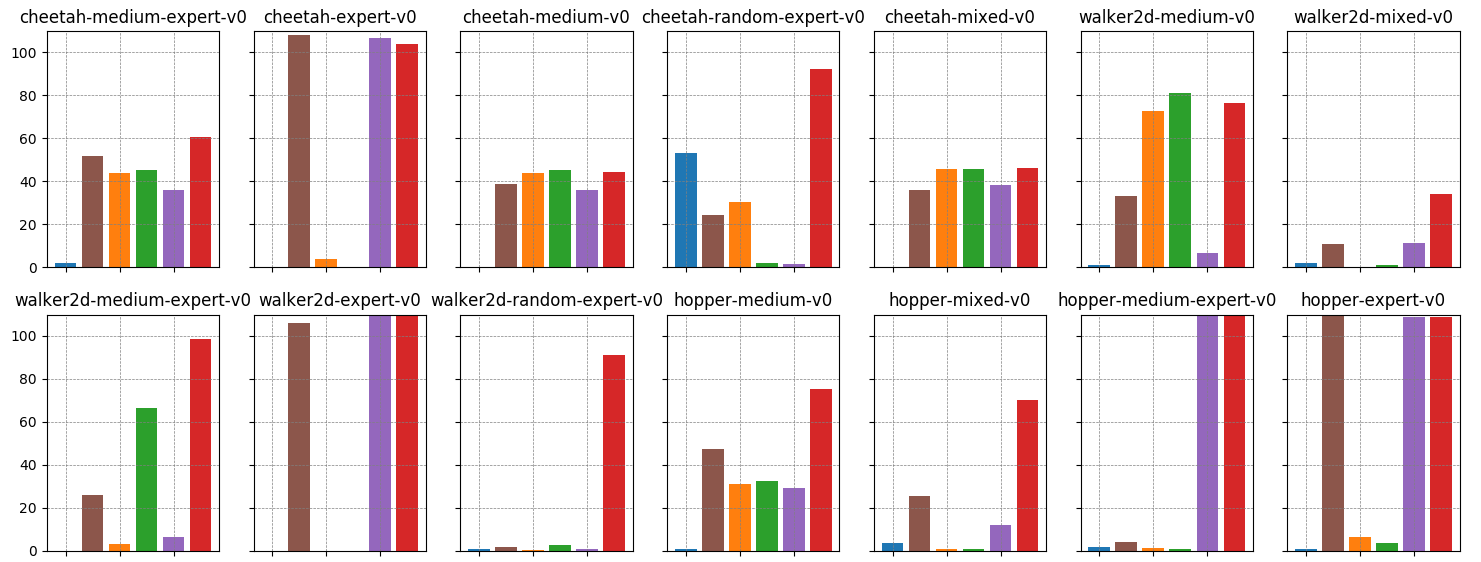
\includegraphics[width=0.99\linewidth]{NeuRIPS2019/images/mujoco_results_v1.png}
% \caption{{\footnotesize Performance of CQL and prior methods on gym MuJoCo tasks from D4RL reported as a normalized score. Observe that CQL performs similarly to the best prior method with simple datasets generated from a single RL policy, and greatly outperforms prior methods with mixed datasets.}}
% \end{figure*}

%% adroit tasks
The more complex Adroit~\citep{rajeswaran2018dapg} tasks (Figure~\ref{fig:d4rl_tasks}) in D4RL require the agent to control a 24-DoF robotic hand, using limited data generated from real-world human demonstrations. These tasks are substantially more difficult than the gym tasks in terms of both the dataset composition and high-dimensionality. Prior offline RL methods generally struggle to learn meaningful behaviors on 
\begin{wrapfigure}{l}{0.55\textwidth}
  \vspace{-18pt}
  \begin{center}
    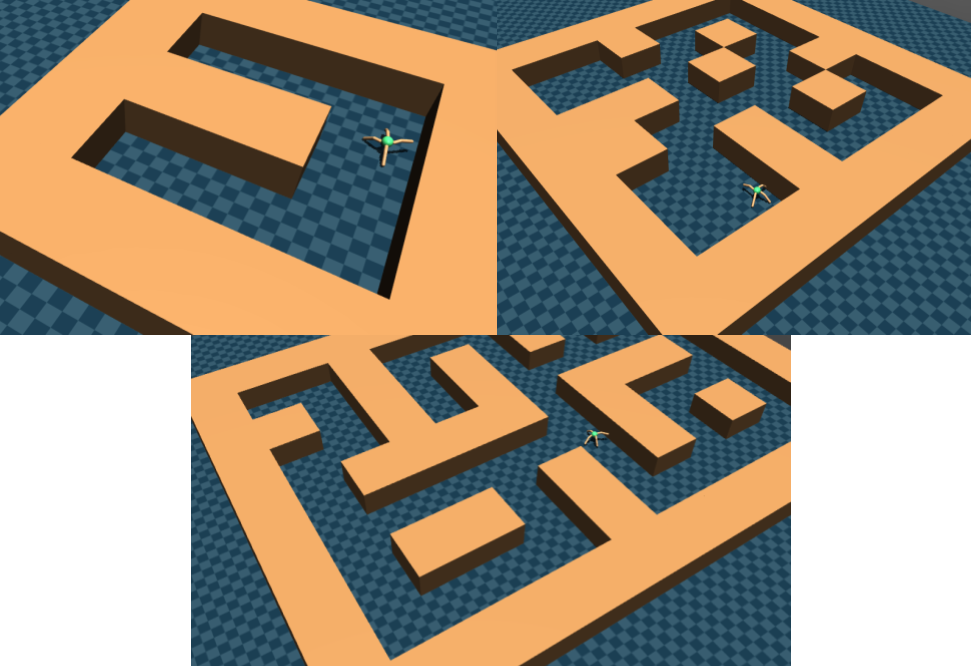
\includegraphics[width=0.2\textwidth]{NeuRIPS2019/images/antmaze_all.png}
    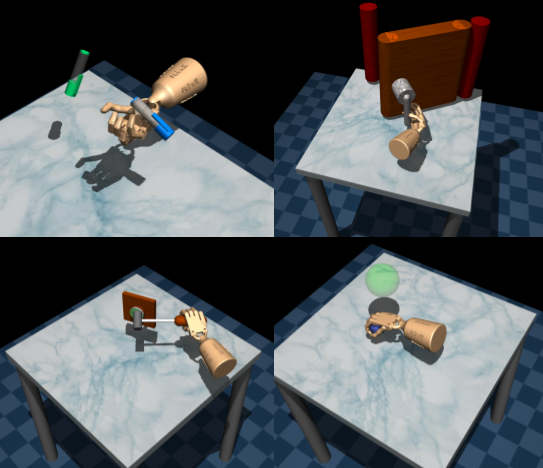
\includegraphics[width=0.16\textwidth]{NeuRIPS2019/images/adroit_all.png}
    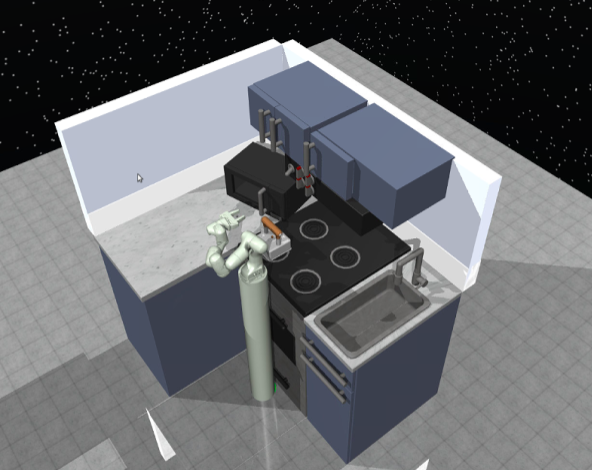
\includegraphics[width=0.17\textwidth]{NeuRIPS2019/images/adept_franka_kitchen.png}
  \end{center}
  \vspace{-7pt}
  \caption{{\small Evaluation tasks in the D4RL suite (from L to R: AntMaze navigation, Adroit, Franka Kitchen tasks).}}
  \vspace{-14pt}
 \label{fig:d4rl_tasks}
\end{wrapfigure}
%%SL.5.24: The spacing here is a little awkward. Also, see my comment about not accidentally releasing results on tasks that don't yet appear in the public D4RL paper!! Also, zoom in on the kitchen a bit, it's really really hard to see what is going on!
these tasks, and the strongest baseline is actually na\"{i}ve behavioral cloning. As shown in Table~\ref{table:adroit_antmaze}, CQL variants are the only methods that improves over na\"{i}ve behavioral
cloning, attaining scores that are \textbf{2-9x} those of the next best offline RL method. As discussed in Section~\ref{sec:framework}, CQL($\rho$), witrh $\rho = \policy^{k}$, i.e. the previous policy, outperforms CQL($\mathcal{H}$) on a number of these adroit tasks, due to the higher action dimensionality resulting in higher variance for the CQL($\mathcal{H}$) importance weights. However, both variants outperform prior methods.
%%AK.5.23: need to say something about the CQL(rho) variant doing better -- which is due to importance sampling, but we never really talk about importance sampling so far.


% When the dataset consists of real-world human demonstrations, as is the case with Adroit tasks~\citep{d4rl}, we observe in Table~\ref{table:adroit_antmaze} that CQL is the only method that is successfully able to outperform the simple BC baseline, and achieves a positive return on all the tasks.
% %%SL.5.11: I would recommend a separate paragraph about Adroit, maybe something like this: The more complex Adroit~\citep{rajeswaran} tasks in D4RL (see Figure ??) require the agent to control a ??-DoF robotic hand, using limited data from real human demonstrations. These tasks are substantially more difficult and high-dimensional than the locomotion tasks described previously. Prior offline RL methods generally struggle to learn meaningful behaviors on these tasks, and the strongest baseline is actually na\"{i}ve behavioral cloning. CQL is the only method that improves over na\"{i}ve behavioral cloning, attaining scores that are ??-??x those of the next best offline RL method.
% %%SL.5.11: can we report normalized scores, so that it's easier to compare? else hard to say if 1000 is really 5x -200...
The maze tasks in D4RL require composing pieces of suboptimal trajectories to form more optimal policies for traveling from a start state to a goal. 
% On the antmaze navigation tasks, shown in Table~\ref{table:adroit_antmaze}, that are specifically designed to test the ability of the underlying offline RL algorithm to compose useful pieces of suboptimal trajectories to solve a task, CQL is the only algorithm that achieves non-trivial performance.
While prior methods sometimes learn meaningful policies on the simpler U-maze, only CQL is able to make meaningful progress on the substantially harder medium and large mazes, achieving nearly \textbf{2-5x} higher return as compared to prior methods.
%%SL.5.11: can we include 2d mazes too? that would help b/c otherwise it looks like something weird is happening with ant maze -- if nothing but our method works, readers might think something is wrong, but if they see 2d maze too, they might realize that ant maze is just harder version of that (showing some images will help!!)
%%SL.5.11: Have a new paragraph for the mazes: The maze tasks in D4RL evaluate more complex data distributions, where an offline RL algorithm must stitch together pieces of trajectories to form optimal policies for traveling from a start state to a goal state, 
% when no direct path between the start and goal is present in the data.
% this condition might be violated for 1-2 envs, so I chose not to write this
% The 2D maze requires navigating a 2D particle through the maze, while the ant mazes require navigating a quadrupedal robot. While prior methods sometimes learn meaningful policies on the simpler 2D mazes, only CQL is able to make meaningful progress on the substantially harder ant mazes, reaching more than half-way to the maximum estimated return in D4RL. In these cases, the final performance of CQL, as compared to the next-best offline RL method, is around 5-10x that of the next-best method.
%%SL.5.11: regarding that 5-10x part: I don't know if this is true -- the table actually reports really high scores for some prior methods, assuming these are out of 1.0? e.g., BEAR is 0.7, but in D4RL I thought it was worse?
%%AK.5.23: Need to add mazes, My maze results are invalid now, since I misunderstood which env to train on, but i have relaunched them and will add them.
% BEAR (and BRAC, too) obtained 0.7 on the easy umaze, which has only one path possible through the maze, even in the D4RL arxiv paper
% but every method was 0 on the two other hard mazes. On maze2d, nothing worked even for the simpler maze (but on ant this was already the case)

Finally, we evaluate CQL on the Franka kitchen domain~\citep{gupta2019relay} from D4RL~\citep{d4rl_repo}.
%%AK.5.23: need to cite the D4RL repo here, since the repo has these tasks, but the paper doesn't yet.
%%SL.5.24: We can go that route, but the subtlety of citing the repo vs the paper will be lost on most people -- I think we have to do this, we need to slightly expand on this point
The goal is to control a 9-DoF robot in a kitchen environment. These tasks require manipulating multiple objects (microwave, kettle, etc.) sequentially in a single episode to reach a desired goal. The agent receives a sparse 0-1 completion reward. These tasks are especially challenging, since they require composing different parts of trajectories, precise long-horizon manipulation, and handling human-provided teleoperation data. As shown in Table~\ref{table:adroit_antmaze}, CQL outperforms prior methods in this setting, and is the only method that outperforms behavioral cloning, attaining over 40\% success rate on all tasks.

%%SL.5.24: Commented out for space constraints
%To summarize, CQL outperforms previous state-of-the-art methods on nearly all of the D4RL tasks, in many cases attaining several times the return of the next best method. This suggests that the relatively simple CQL regularizer has the potential to improve offline RL performance.


\begin{table}[]
\centering

%\scriptsize
\fontsize{8}{8}\selectfont

\begin{tabular}{l|l|r|r|r|r|r||r|r}
\hline
\textbf{Domain} & \textbf{Task Name} & \textbf{BC} & \textbf{SAC} & \textbf{BEAR} & \textbf{BRAC-p} & \textbf{BRAC-v} & \textbf{CQL($\mathcal{H}$)} & \textbf{CQL($\rho$)}\\ \hline
% \multirow{3}*{Maze2D}
% & maze2d-umaze &  3.8 & 88.2 & 3.4 & 4.7 & -14.6\\
% & maze2d-medium &  30.3 & 26.1 & 29.0 & 32.4 & 149.0\\
% & maze2d-large &  5.0 & -1.9 & 4.6 & 10.4 & 150.0\\
% \hline
\multirow{6}*{AntMaze}
& antmaze-umaze & 65.0 & 0.0 & \textbf{73.0} & 50.0 & 70.0 & \textbf{74.0} & \textbf{73.5}\\
& antmaze-umaze-diverse  & 55.0 & 0.0 & 61.0 & 40.0 & 70.0 & \textbf{84.0} & 61.0\\
& antmaze-medium-play  & 0.0 & 0.0 & 0.0 & 0.0 & 0.0 & \textbf{61.2} & 4.6 \\
& antmaze-medium-diverse  & 0.0 & 0.0 & 8.0 & 0.0 & 0.0 & \textbf{53.7} & 5.1 \\
& antmaze-large-play & 0.0 & 0.0 & 0.0 & 0.0 & 0.0 & \textbf{15.8} &  3.2\\
& antmaze-large-diverse & 0.0 & 0.0 & 0.0 & 0.0 & 0.0 & \textbf{14.9} & 2.3 \\
\hline
\multirow{8}*{Adroit}
& pen-human  & 34.4 & 6.3 & -1.0 & 8.1 & 0.6 & 37.5 & \textbf{55.8}\\
& hammer-human & 1.5 & 0.5 & 0.3 & 0.3 & 0.2 & \textbf{4.4} & {2.1}\\
& door-human & 0.5 & 3.9 & -0.3 & -0.3 & -0.3 & \textbf{9.9} & \textbf{9.1} \\
& relocate-human & 0.0 & 0.0 & -0.3 & -0.3 & -0.3 & 0.20 & \textbf{0.35}\\
& pen-cloned  & \textbf{56.9} & 23.5 & 26.5 & 1.6 & -2.5 & 39.2 & 40.3\\
& hammer-cloned & 0.8 & 0.2 & 0.3 & 0.3 & 0.3 & 2.1 & \textbf{5.7} \\
& door-cloned & -0.1 & 0.0 & -0.1 & -0.1 & -0.1 & 0.4 & \textbf{3.5}\\
& relocate-cloned & \textbf{-0.1} & -0.2 & -0.3 & -0.3 & -0.3 & \textbf{-0.1} & \textbf{-0.1}\\
\hline
\multirow{3}*{Kitchen}
& kitchen-complete & 33.8 & 15.0 & 0.0 & 0.0 & 0.0 & \textbf{43.8} & 31.3\\
& kitchen-partial & 33.8 & 0.0 & 13.1 & 0.0 & 0.0 & \textbf{49.8} & \textbf{50.1} \\
& kitchen-undirected & 47.5 & 2.5 & 47.2 & 0.0 & 0.0 & \textbf{51.0} & \textbf{52.4} \\ \hline
\end{tabular}
\normalsize
\caption{\label{table:adroit_antmaze}{\small Normalized scores of all methods on AntMaze, Adroit, and kitchen domains from D4RL, averaged across 4 seeds. On the harder mazes, CQL is the \textit{only} method that attains non-zero returns, and is the only method to outperform simple behavioral cloning on Adroit tasks with human demonstrations.
The CQL($\rho$) variant, which avoids importance weights, is more stable on the higher-dimensional Adroit tasks.}}
\vspace{-25pt}
\end{table}

% \begin{table*}[h]
% \centering
% \small
% \begin{tabular}{l|r|r|r|r|r|r|r|r}
% \hline
% \textbf{Task Name} & \textbf{SAC} & \textbf{BC} & \textbf{SAC-off} & \textbf{BEAR} & \textbf{BRAC-p} & \textbf{BRAC-v} & \textbf{CQL($\mathcal{H}$)} & \textbf{CQL($\rho$)}\\ \hline
% ant-umaze & 0.0 & 0.7 & 0.0 & 0.7 & 0.5 & 0.7 & \textbf{0.74} & \\
% ant-umaze-diverse & 0.0 & 0.6 & 0.0 & 0.6 & 0.4 & 0.7 & \textbf{0.79} & \\
% ant-medium-play & 0.0 & 0.0 & 0.0 & 0.0 & 0.0 & 0.0 & \textbf{0.54 } & \\
% ant-medium-diverse & 0.0 & 0.0 & 0.0 & 0.0 & 0.0 & 0.0 & \textbf{0.53} & \\
% ant-large-play & 0.0 & 0.0 & 0.0 & 0.0 & 0.0 & 0.0 & \textbf{0.20} & \\
% ant-large-diverse & 0.0 & 0.0 & 0.0 & 0.0 & 0.0 & 0.0 & \textbf{0.19} & \\
% \hline
% pen-human & 739.3 & 1121.9 & 284.8 & 66.3 & 339.0 & 114.7 & \textbf{1367.5} & \\
% hammer-human & -248.7 & -82.4 & -214.2 & -242.0 & -239.7 & -243.8 & \textbf{1098.1} & \\
% door-human & -61.8 & -41.7 & 57.2 & -66.4 & -66.5 & -66.4 & \textbf{273.0} & \\
% relocate-human & -13.7 & -5.6 & -4.5 & -18.9 & -19.7 & -19.7 & \textbf{5.7} & \\
% pen-cloned & \\
% hammer-cloned & \\
% door-cloned & \\
% relocate-cloned & \\
% \hline
% mini-kitchen-MKLS & \\
% kitchen-MKLS & \\
% kitchen-MKBL & \\
% \hline
% \end{tabular}
% \caption{{\footnotesize Performance of CQL and prior methods on AntMaze, Adroit and kitchen tasks from D4RL. Observe that CQL outperforms prior methods on the simpler U-shaped maze and is the \textit{only} method that is able to obtain non-zero performance on the harder, medium-sized maze. CQL is the only method that achieves a positive return on adroit tasks with human demonstrations.}}
% \label{table:adroit_antmaze}
% \normalsize
% \end{table*}
% \multirow{12}*{Adroit}
% & pen-human & 739.3 & 1121.9 & 284.8 & 66.3 & 339.0 & 114.7\\
% & pen-cloned & 739.3 & 1791.8 & 797.6 & 885.4 & 143.4 & 22.2\\
% & pen-expert & 739.3 & 2633.7 & 277.4 & 3254.1 & -7.8 & 6.4\\
% & hammer-human & -248.7 & -82.4 & -214.2 & -242.0 & -239.7 & -243.8\\
% & hammer-cloned & -248.7 & -175.1 & -244.1 & -241.1 & -236.7 & -236.9\\
% & hammer-expert & -248.7 & 16140.8 & 3019.5 & 16359.7 & -241.4 & -241.1\\
% & door-human & -61.8 & -41.7 & 57.2 & -66.4 & -66.5 & -66.4\\
% & door-cloned & -61.8 & -60.7 & -56.3 & -60.9 & -58.7 & -59.0\\
% & door-expert & -61.8 & 969.4 & 163.8 & 2980.1 & -66.4 & -66.6\\
% & relocate-human & -13.7 & -5.6 & -4.5 & -18.9 & -19.7 & -19.7\\
% & relocate-cloned & -13.7 & -10.1 & -16.1 & -17.6 & -19.8 & -19.4\\
% & relocate-expert & -13.7 & 4289.3 & -18.2 & 4173.8 & -20.6 & -21.4\\
% \hline
% \multirow{12}*{Gym}
% & halfcheetah-random & 12135.0 & -17.9 & 3502.0 & 2885.6 & 2641.0 & 3207.3\\
% & halfcheetah-medium & 12135.0 & 4196.4 & -808.6 & 4508.7 & 5178.2 & 5365.3\\
% & halfcheetah-mixed & 12135.0 & 4492.1 & -581.3 & 4211.3 & 5384.7 & 5413.8\\
% & halfcheetah-medium-expert & 12135.0 & 4169.4 & -55.7 & 6132.5 & 5156.0 & 5342.4\\
% & walker2d-random & 4592.3 & 73.0 & 192.0 & 307.6 & 38.4 & 23.9\\
% & walker2d-medium & 4592.3 & 304.8 & 44.2 & 1526.7 & 3341.1 & 3734.4\\
% & walker2d-mixed & 4592.3 & 518.6 & 87.8 & 495.3 & -11.5 & 44.5\\
% & walker2d-medium-expert & 4592.3 & 297.0 & -5.1 & 1193.6 & 141.7 & 3058.9\\
% & hopper-random & 3234.3 & 299.4 & 347.7 & 289.5 & 341.0 & 370.5\\
% & hopper-medium & 3234.3 & 923.5 & 5.7 & 1527.9 & 994.8 & 1030.0\\
% & hopper-mixed & 3234.3 & 364.4 & 93.3 & 802.7 & 2.0 & 5.3\\
% & hopper-medium-expert & 3234.3 & 3621.2 & 32.9 & 109.8 & 16.0 & 5.1\\
% \hline

%%SL.5.24: Consider deleting subsection headings in the whole experiments section. They really don't add much, and you can save some space.
%\subsection{Offline Image-Based RL on the Arcade Learning Environment}
Lastly, we evaluate a discrete-action Q-learning variant of CQL (Algorithm~\ref{alg:practical_alg}) on image-based Atari games~\citep{bellemare2013arcade}. We compare CQL to REM~\citep{agarwal2019optimistic} and QR-DQN~\citep{dabney2018distributional} on the four Atari tasks that are evaluated in detail by \citet{agarwal2019optimistic}, using the dataset released by the authors: Pong, Breakout, Qbert and Seaquest. We were not able to reproduce the QR-DQN and REM results on Asterix using the official implementation and data from \citet{agarwal2019optimistic}, and no method was able to perform well on the provided data for this task, but we include the scores in Table~\ref{table:atari_reduced_size}.
\begin{figure*}[h]
\vspace{-10pt}
  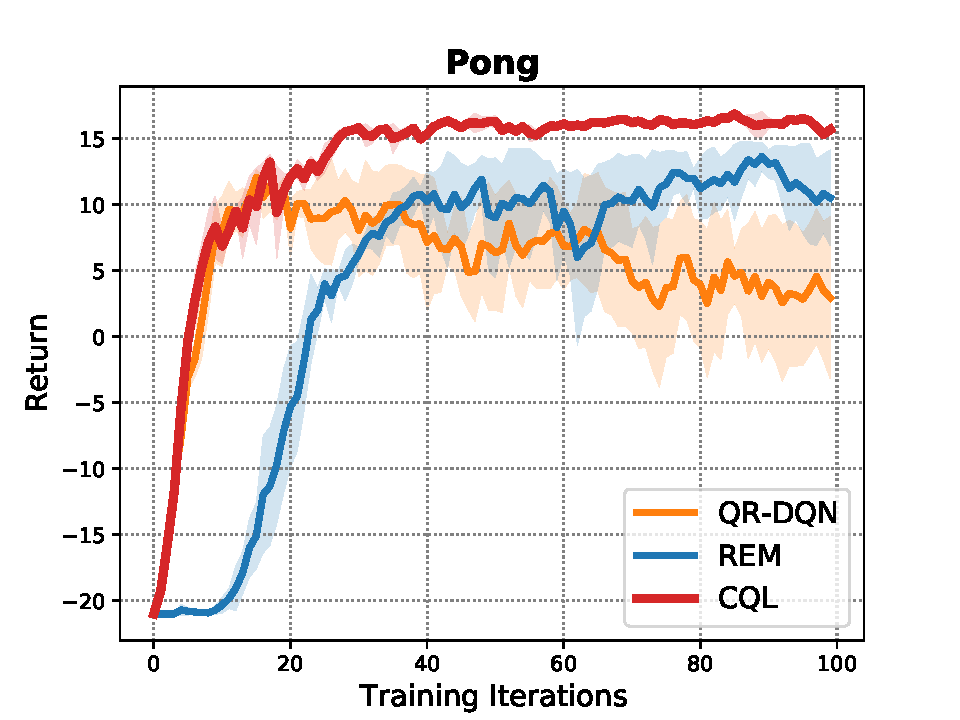
\includegraphics[width=0.23\linewidth]{NeuRIPS2019/images/pong.pdf}  
  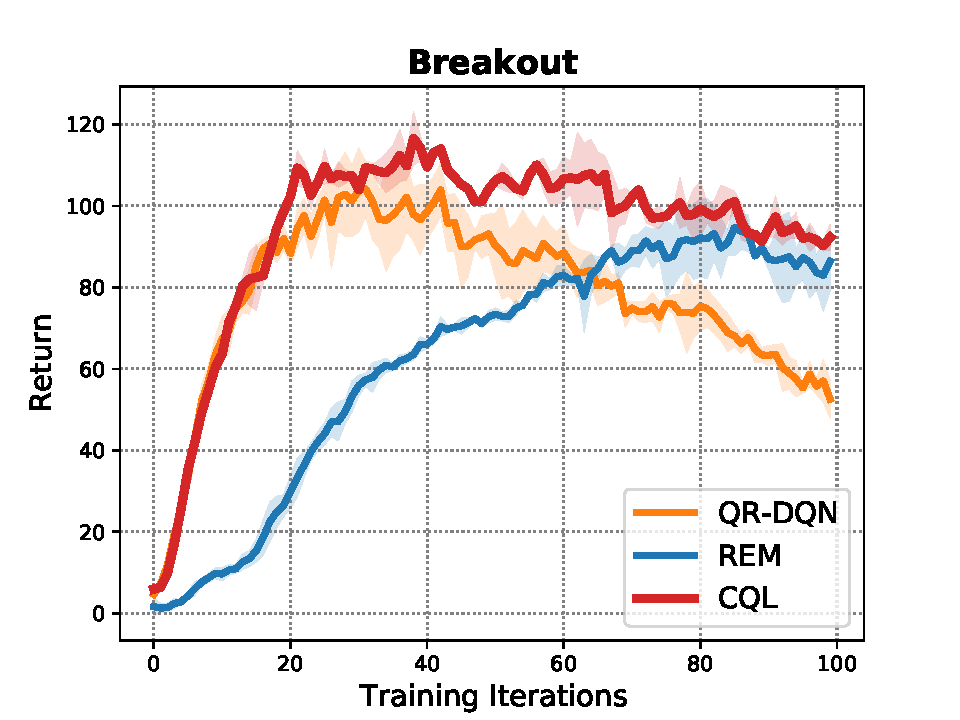
\includegraphics[width=.23\linewidth]{NeuRIPS2019/images/breakout.pdf}  
  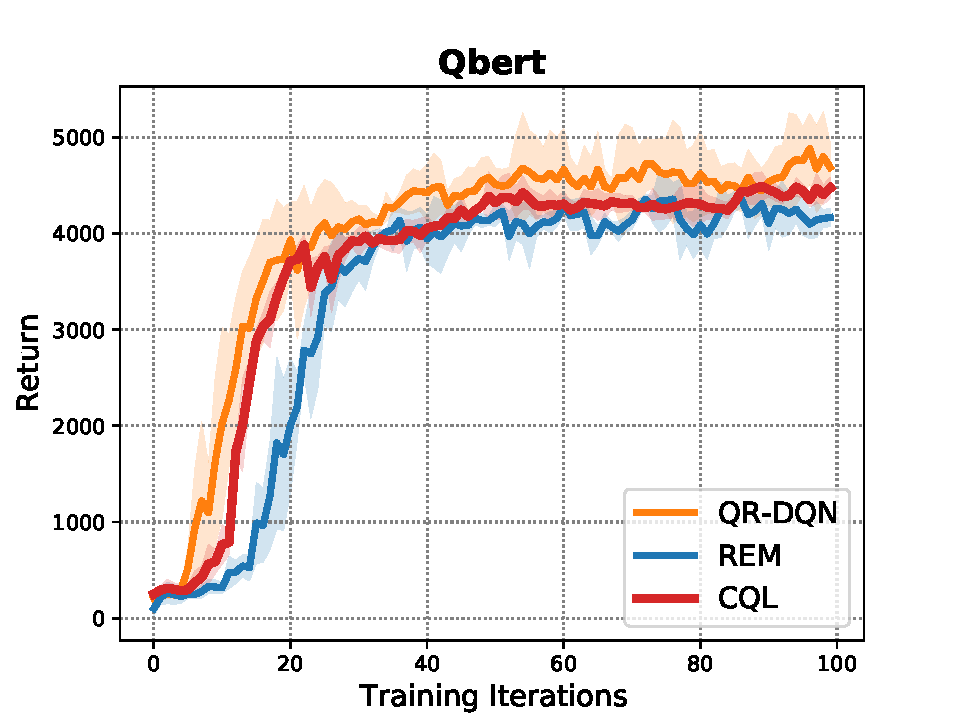
\includegraphics[width=.23\linewidth]{NeuRIPS2019/images/qbert.pdf}  
  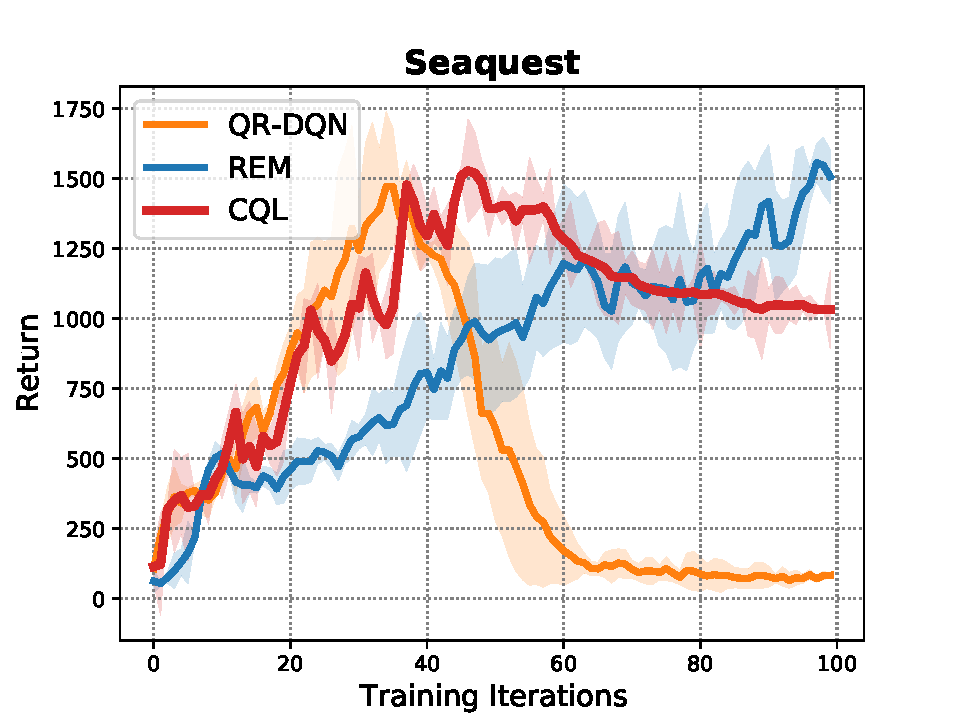
\includegraphics[width=.23\linewidth]{NeuRIPS2019/images/seaquest.pdf}  
\caption{\label{fig:cql_20m_atari}{\footnotesize Performance of CQL, QR-DQN and REM as a function of training steps (x-axis) in setting \textbf{(2)} when provided with only the first 20\% of the samples of an online DQN run. Note that CQL is able to learn stably on 3 out of 4 games, and its performance does not degrade as steeply as QR-DQN on Seaquest.}}
\vspace{-10pt}
\end{figure*}
Following the evaluation protocol of \citet{agarwal2019optimistic}, we evaluated on two types of datasets, both of which were generated from the DQN-replay dataset:
\textbf{(1)} a dataset consisting of the first 20\% of the samples observed by an online DQN agent (Fig. 7 in \citep{agarwal2019optimistic}) and 
\textbf{(2)} datasets consisting of only 1\%  and 10\% of the samples in the replay buffer of an online DQN agent (Fig. 6 in \citep{agarwal2019optimistic}). In setting \textbf{(1)}, shown in Figure~\ref{fig:cql_20m_atari}, CQL generally achieves similar or better performance over the course of training as QR-DQN and REM.
%AK: TODO (aviral): revisit this if we can't get seaquest to work -- Seaquest is almost maxed out, need to decide on what to say here?
When only using only 1\% or 10\% of the data, in setting \textbf{(2)}, we see in Table~\ref{table:atari_reduced_size} that CQL substantially outperforms REM and QR-DQN, especially in the harder 1\% condition, where performance exceeds the best prior method by as much as \textbf{28x} on Q*bert, and \textbf{6x} on Breakout.
% don't say this last part unless we have evidence specifically for this
%%SL.5.11: I would just omit saying this last part regardless, I don't think it adds much and just confuses the reader.
% done
% In setting \textbf{(2)}, shown in Figure~\ref{fig:cql_20m_atari}, CQL achieves similar or better performance and is more stable as compared to prior methods. 
% TODO (aviral): try harder on seaquest, it is still better than QR-DQN and REM, but see if we can avoid the drop, possibly using lagrange optimization. 
%%SL.5.11: Maybe what we should do if CQL is about the same in (2), is just reverse them: first present (2) (call it (1)), and say: in this setting, CQL matches the prior methods. However, when using just 1\% or 10\% of the data, in condition (2), CQL outperforms the prior methods drastically, especially in the harder 1\% condition, where performance exceeds prior methods by as much as 28x (on Q*bert), and is ?? times higher on average across the games compared to the next best method.
% done

\begin{table}[h]
    \centering
    \begin{tabular}{l|r|r|r|||r|r|r}
    \hline
        \textbf{Task Name} & \textbf{QR-DQN} & \textbf{REM} & \textbf{CQL($\mathcal{H}$)}  & \textbf{QR-DQN} & \textbf{REM} & \textbf{CQL($\mathcal{H}$)}  \\
        \hline
         Pong & 3.0 & 6.0 & \textbf{19.3} & 16.7 & 16.8 & \textbf{18.5} \\
         Breakout & 7.8 & 9.2 & \textbf{61.1} & 176.0 & 96.0 & \textbf{269.3} \\
         Q*bert & 500.0 & 500.0 & \textbf{14012.0}& 11201.8 & 8070.2 & \textbf{13855.6}\\
         Seaquest & 480.2 & 390.1 & \textbf{779.4} & 3300.0 & \textbf{4290.4} & 3674.1 \\
         Asterix\footnote{No method (CQL or prior methods, REM and QR-DQN, were able to attain non-trivial performance on this game using the dataset provided by \citet{agarwal2019optimistic}} & 166.3 & 386.5 & \textbf{592.4} & 189.2 & 75.1 & 156.3 \\
         %%SL.5.27: can you add a footnote on Asterix, and write: Note that no method (ours or prior) was able to attain non-trivial performance on this task using the dataset provided by \citet{agrawal}.
         \hline
    \end{tabular}
    \caption{{\footnotesize CQL, REM and QR-DQN in setting \textbf{(1)} with 1\% data (left), and 10\% data (right). CQL drastically outperforms prior methods with 1\% data, and usually attains better performance with 10\%.}}
    \label{table:atari_reduced_size}
\end{table}


%%AK.5.23: Commenting out this for now, discussion in the email. Basically we are not doing great here especially with the right way of using the Q-values for computing policy return. It is conservative, but it is too conservative in 4/8 cases (like the method outputs 153.4 as the return, but the actual return is 276). I think that if we believe that the other story is storng enough, we should probably not have it.
% \subsection{Off-Policy Evaluation Experiments}

% %%SL.5.11: Can we start off with a little transition to explain why we're talking about this? E.g., something like: The core of CQL is a Q-function learning method that learns a lower bound on the true Q-function. This lower bound can be used to learn a better policy, or simply to evaluate an existing policy. In this section, we study this latter setting, applying CQL to the off-policy evaluation problem.
% % done
% CQL learns a Q-function such that the expected value of the policy under this learned Q-function lower-bounds the true policy value. In this section, we evaluate the performance of CQL for evaluating the performance of a pre-specified policy using pre-specified offline datasets on three continuous control domains: Hopper, HalfCheetah and Walker2d. In accordance with the setup in prior work~\citep{Zhang2020GenDICE}, our task is to evaluate the return of an expert SAC policy using data generated from a mixture of suboptimal policies. Thus, we use the medium-expert and mixed datasets from \citep{d4rl} that contain a diverse mixture of suboptimal policies as the offline datasets.

% We compare CQL to state-of-the-art prior method, GenDICE~\citep{zhang2019generalized}, in Table ??. Note that CQL learns conservative return estimates, that lower bound the actual discounted return of the target policy, thus empirically validating the theoretical insights discussed in Section~\ref{sec:policy_eval}. In contrast,  (One line about OTHER METHODS once we have numbers) \ak{TODO: put table.}
